
\chapter{Gamma-ray Astrophysics}
\chaplabel{gamma_ray_astro}

\section{Astronomy and the Atmosphere}
\seclabel{astronomy_and_the_atmosphere}

Humans surely have, since the very beginning,
 stared into space and contemplated its brilliance.
Stone circles in the Nabta Playa in Egypt are likely the first observed
astronomical observatory and are believed to have acted as a prehistoric
calendar.  Dating back to the 5th century BC, they are 1,000 years older
than stonehenge \citep{mck-mahille_2007_astronomy-nabta}.  

\begin{figure}[htb]
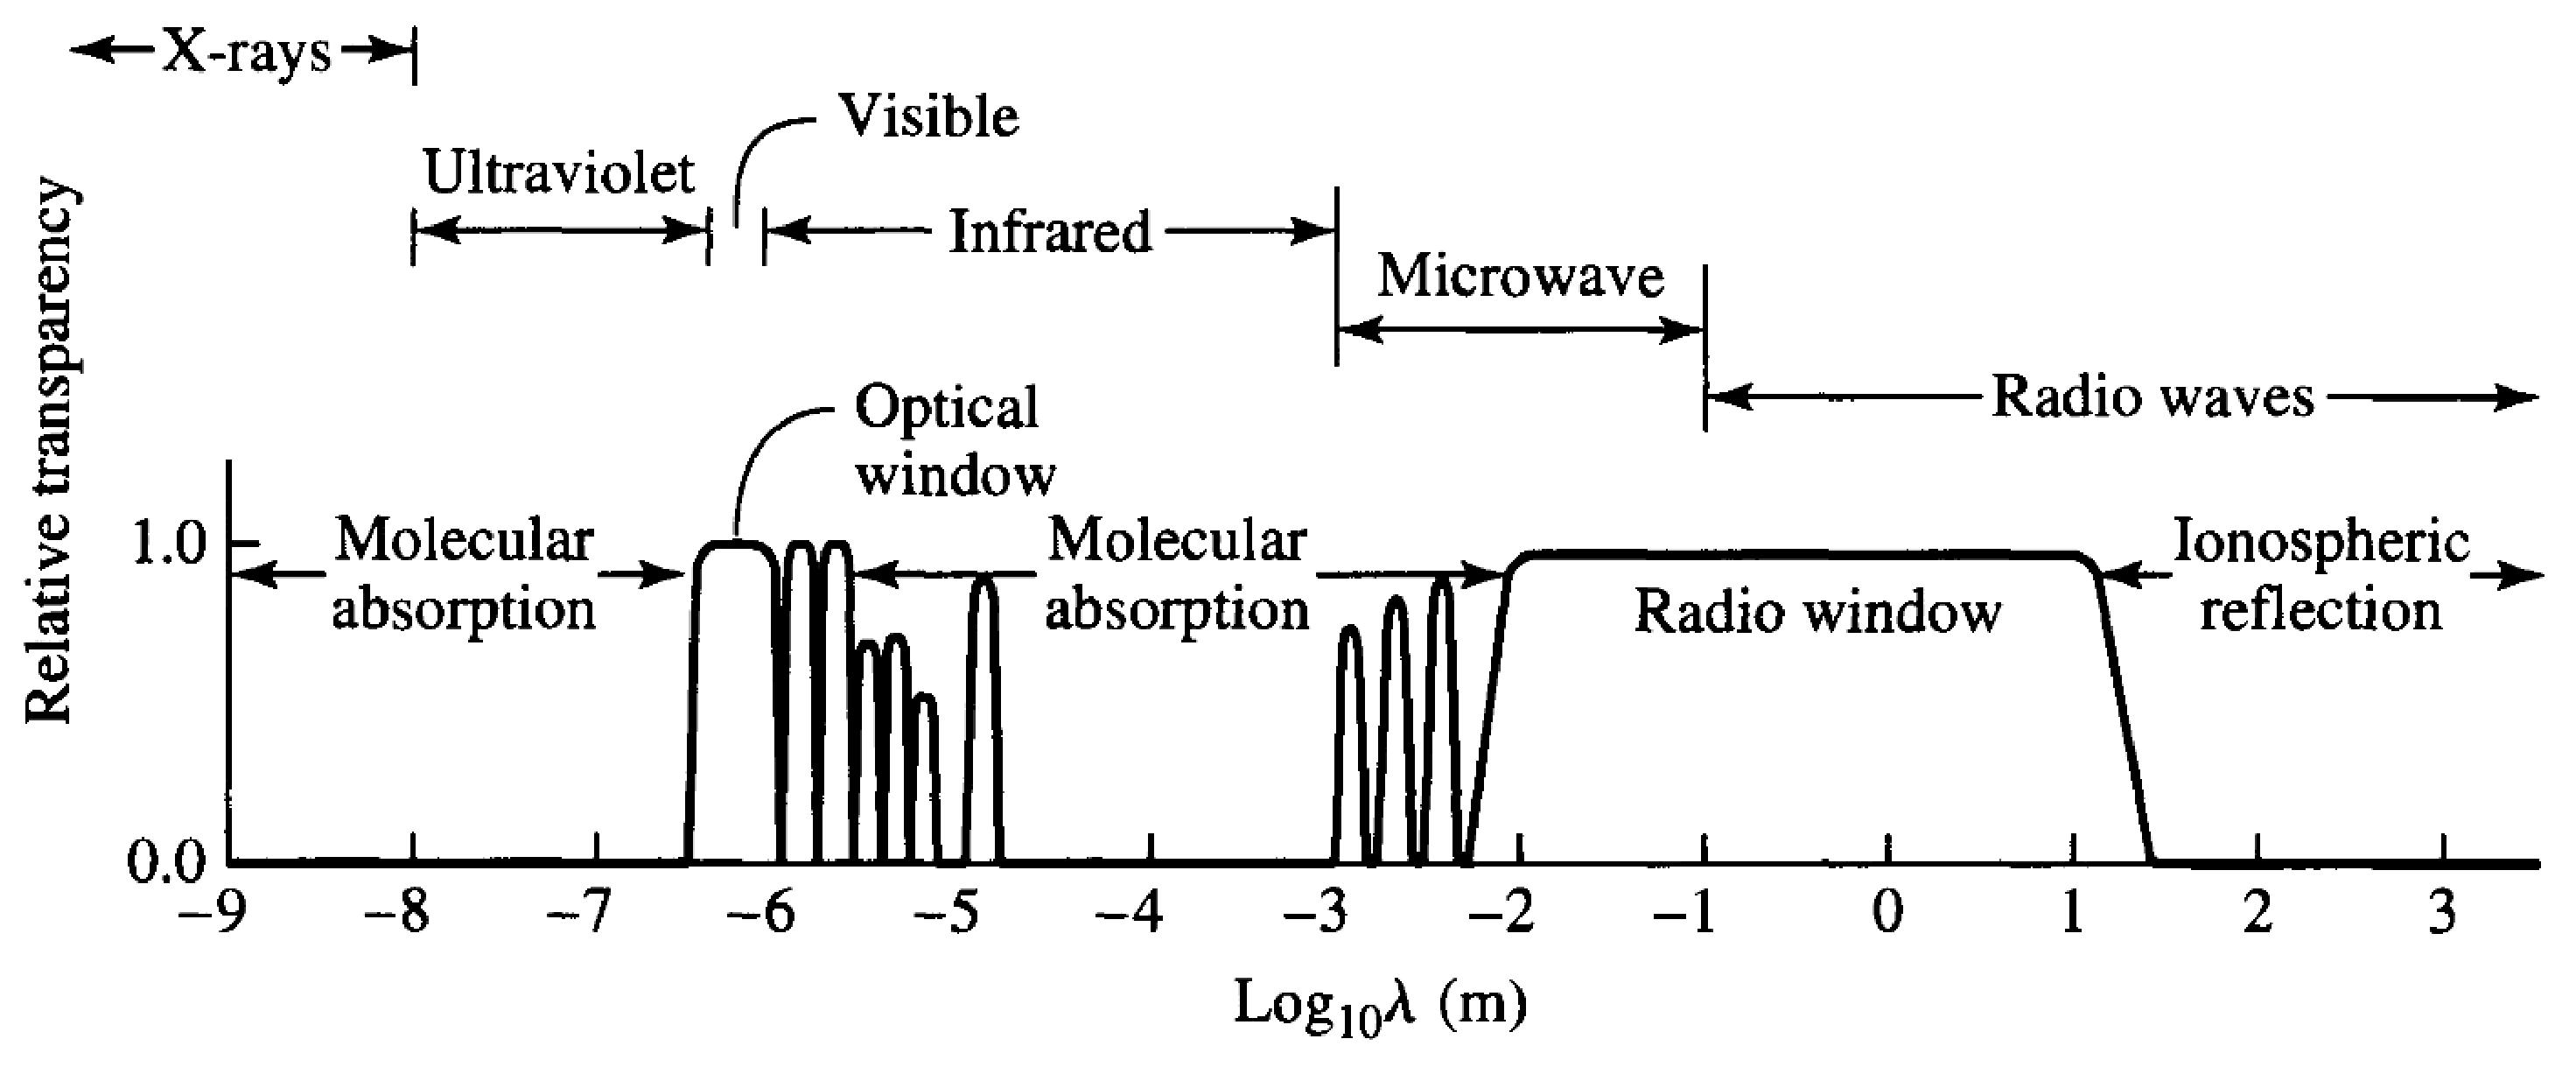
\includegraphics[width=\textwidth]{chapters/introduction/figures/atmospheric_absorption.pdf}
\figlabel{atmospheric_absorption}
\caption{
Transparency of the atmosphere of the earth to photons of 
varying wavelenthts.  This figure is from \cite{carroll_2006_introduction-modern}
}
\end{figure}

% Thorough discussion of all experiments:
%   http://imagine.gsfc.nasa.gov/docs/sats_n_data/gamma_missions.html
%   http://space.about.com/od/telescopesandoptics/a/Gammaray-Astronomy.htm

% Nice history with lots of pictures:
%  http://fermi.gsfc.nasa.gov/science/mtgs/symposia/2012/program/mon/DKniffen.pdf

% Good books with introduction

%  "Very High Energy Gamma Ray Astronomy" by Trevor C. Weekes
%    * seems to have a discussion of the principles of Gamma-ray detection.
%      scintilation detectors, spark chambers.

%  "Cosmic Gamma-Ray Sources" - edited by K.S. Cheng, Gustavo E. Romero

% Very nice reference:
%   http://adsabs.harvard.edu/abs/1984BASI...12..202P

% Nice summary:
%   http://articles.adsabs.harvard.edu/cgi-bin/nph-iarticle_query?1984BASI...12..202P&amp;data_type=PDF_HIGH&amp;whole_paper=YES&amp;type=PRINTER&amp;filetype=.pdf

Astronomy has historically been almost entirely concerned with studying
the photons that arrive from outer space.  Because of their charge
neutrality, photons are not defected by intergalactic electric and
magnetic fields and therefore point back to the objects 
emitting them. 

Historically, the field of astronomy concerned
the study of visible light. The reason for this is visible light
is not signifcantly absorbed in the atmosphere. 
In addition to the visible spectrum, radio waves, some
energies of infrared radiation, and long-wavelenth ultraviolet
radiation can be measured from the ground. Figure
\figref{atmospheric_absorption} shows the transparancy
of the atmosphere of the earth to photons of differnet wavelenths.

Slowly, over time, astronomers expanded their view across the
electromagnetic spectrum.  First, the astronomical observations
were made from the ground.  Infrared radiation from the sun was
first observed by William Herschel in 1800. Herschel measured this
infrared radiation by measuring the temperature of sunlight through
a prisim and extending the measurement past the red part of the
spectrum \citep{herschel_1800_experiments-refrangibility}.  The first
extraterrestrial source of radio waves was detected by Jansky in 1933.
Janksy, a radio engineer at Bell labs, was studying the
origins of radio interference when he detected radio emission towards
the center of our galaxy.
\citep{jansky_1933_electrical-disturbances}.

% x-ray: http://en.wikiversity.org/wiki/Radiation_history#cite_ref-Burnight_183-1
The expansion of the astronomical fronteire to other wavelenths required
the development of rockets and sattelites in the 20th ceuntry.  The first
ultraviolet observation of the sun was performed in 1946 from a captured
V-2 rocket \citep{baum_1946_ultraviolet-spectrum}.  Observations of
solar x-rays were also first carried out on a captured V-2 Rocket in
1949 \citep{burnight_1949_x-radiation-atmosphere}.



\section{The History of Gamma-ray Astrophysics}
\seclabel{history_gamma_ray_detectors}

% Thorough discussion of all experiments:
%   http://imagine.gsfc.nasa.gov/docs/sats_n_data/gamma_missions.html
%   http://space.about.com/od/telescopesandoptics/a/Gammaray-Astronomy.htm

% Nice history with lots of pictures:
%  http://fermi.gsfc.nasa.gov/science/mtgs/symposia/2012/program/mon/DKniffen.pdf

% Good books with introduction

%  "Very High Energy Gamma Ray Astronomy" by Trevor C. Weekes
%    * seems to have a discussion of the principles of Gamma-ray detection.
%      scintilation detectors, spark chambers.

%  "Cosmic Gamma-Ray Sources" - edited by K.S. Cheng, Gustavo E. Romero

% Very nice reference:
%   http://adsabs.harvard.edu/abs/1984BASI...12..202P

% Nice summary:
%   http://articles.adsabs.harvard.edu/cgi-bin/nph-iarticle_query?1984BASI...12..202P&amp;data_type=PDF_HIGH&amp;whole_paper=YES&amp;type=PRINTER&amp;filetype=.pdf

Astronomy has historically been almost entirely concerned with studying
the photons that arrive from outer space.  Because of their charge
neutrality, photons are not defected by intergalactic electric and
magnetic fields and therefore point back to the objects 
emitting them. Historically, the field of astronomy concerned
the study of visible light.  Slowly, over time, astronomers 
expanded their view across the electromagnetic spectrum.

Infrared radiation from the sun was first observed by
William Herschel in 1980 \citep{herschel_1800_experiments-refrangibility}.
The first extraterrestrial source of radio waves was detected
by Jansky in 1933 \citep{jansky_1933_electrical-disturbances}.

% x-ray: http://en.wikiversity.org/wiki/Radiation_history#cite_ref-Burnight_183-1
The development of rockets and sattelites in the 20th ceuntry allowed
the field of astronomy to expand futher, allowering observations
at wavelengths that would otherwise be absorbed in the atmosphere.
The first ultraviolet observation of the sun was performed in 1946 from a
captured V-2 rocket \citep{baum_1946_ultraviolet-spectrum}.  Observations of
solar x-rays were also first carried out on a captured V-2 Rocket in
1949 \citep{burnight_1949_x-radiation-atmosphere}

It was only natural to wonder about the universe at even higher energies.
As is common in the field of physics, the prediction of
the detection of cosmic $\gamma$-rays far proceded their discovery.
\cite{feenberg_1948_interaction-cosmic-ray} theorized that the interaction
of starlight with cosmic rays could produce $\gamma$-rays through
\ac{IC} upscattering.  Following the discovery of the neutral
pion in 1949, \cite{hayakawa_1952_propagation-cosmic}
predicted that $\gamma$-ray emission could be observed from the
decay of neutral pions when cosmic rays interacted with interstellar
matter.  And in the same year, \cite{hutchinson_1952_possible-relation}
discussed the bremsstrahlung radiation of cosmic-ray electrons.
\cite{morrison_1958_gamma-ray-astronomy} first predicted the detection
of several sources of $\gamma$-rays including solar flares, \acp{PWN},
and active galaxies.

\todo[inline]{
Why Gamma-rays can't make it to the ground
}
    
\todo[inline]{Discuss
Balloon gamma-ray detectors.
See discussion on p859 (comparison with other 
experiments) of Kraushaar et al 1965. 
What was the background from, earth albedo gammas I think?
See also Kraushaar et al 1972 p342's discussion of the balloon
experiments: Hulsizer and Rossi (1949), ... 
See also William Tomkin's section 2.2.1 on 
Balloon experiments (page 8) for references
to galactic plane emission being measured
by balloon experiments in 1970.}


    % Links on Explorer 11
% en.wikipedia.org/wiki/Explorer_11
%http://www.physics.wisc.edu/news/obits/kraushaar_obit.html
% http://heasarc.nasa.gov/docs/heasarc/missions/explorer11.html#reference
% http://articles.adsabs.harvard.edu/cgi-bin/nph-iarticle_query?1965ApJ...141..845K&amp;data_type=PDF_HIGH&amp;whole_paper=YES&amp;type=PRINTER&amp;filetype=.pdf

% "The instrument package weighed 30 pounds, was 20 inches high and 10 inches in diameter. The experimenters believed that they detected 22 cosmic gamma rays."
%  -> http://imagine.gsfc.nasa.gov/docs/sats_n_data/gamma_missions.html
The first space-based $\gamma$-ray detector was \explorerxi
\cite{kraushaar_1965_explorer-experiment}.  It was developed at \ac{MIT}
under the direction of William L. Kraushaar.  It employed a sandwich
scintillator and a Cherenkov counter to direct the position and energy
of incoming $\gamma$-rays and was surounded by a plastic anticoincidence
scintilation counter. The sandwich detector had an area of $\sim45\cm^2$,
but an effective area of only $\sim 7\cm^2$, corresonding
to a detector efficiency of $\sim 15\%$.

\todo[inline]{What was the energy range of explorer ii}

It was launched on boad \explorerxi on April 27,
1961. The instrument was in opreation for 7 months, but only 141 hours
of data were of acceptable quality.  Using these observations, \explorerxi
observed 31 $\gamma$-rays and, because the distribution a distribution of
these $\gamma$-rays was consistent with being isotropic, the experiment
could not firmly identify the $\gamma$-rays as being cosmic in nature.


% en.wikipedia.org/wiki/OSO_3
% "Their
% next detector, on Orbiting Solar Observatory -3, may be more accurately
% described as having proof of the discovery of cosmic gamma radiation,
% since it found a galactic plane anisotropy of high-energy gammas, much
% later to be confirmed with SAS-2 and COS-B." -- http://imagine.gsfc.nasa.gov/docs/sats_n_data/gamma_missions.html

% Notes: 621 photons, E>100 GeV, 1967, angular resolution +/- 16deg from 
%  ``Cosmic Gamma-Ray Sources`` K.S. Chen, Gustavo E. Romer

\todo[inline]{Describe scintilation detector better.
Read William Tomkin's thesis, page 8.}

The first definitive detection of $\gamma$-ray came in
1962 by an experiment on the Ranger 3 moon
probe \citep{arnold_1962_gamma-space}.  It detected an isotropic flux
of $\gamma$-rays in the 0.5 \mev to 2.1 \mev energy range.

\ac{OSO-3}, also developed by Kraushaar, followed \explorerxi
as the next major astrophysical $\gamma$-ray detector
\cite{kraushaar_1972_high-energy-cosmic}.  The \ac{OSO-3} sattelite
allowed the on board $\gamma$-ray detected to have an improved weight,
power, telemetry, and expsoure, creating a more sensitive experiment.
The experiment operated in the energy range from 50 \mev to $\sim 400$
\mev and had an effective area $\sim 9$ $\cm^2$.

It was launched on March 8, 1967 and operated for 16 months, measuring
621 cosmic $\gamma$-rays.  The most important result of the expirment was
to measure a strong anisotrophy in the distribution of the $\gamma$-rays
with a strong clustering of $\gamma$-rays towards the Galactic plane.
\figref{oso3_skymap} shows a skymap of these $\gamma$-rays.  This
experiment confirmed both a Galactic component to the $\gamma$-ray
sky as well as an additional isotropic component, hypothesised to be
extragalactic in origin.

\todo[inline]{What was the PSF of OSO-3? could it be pointed?}

\begin{figure}[htb]
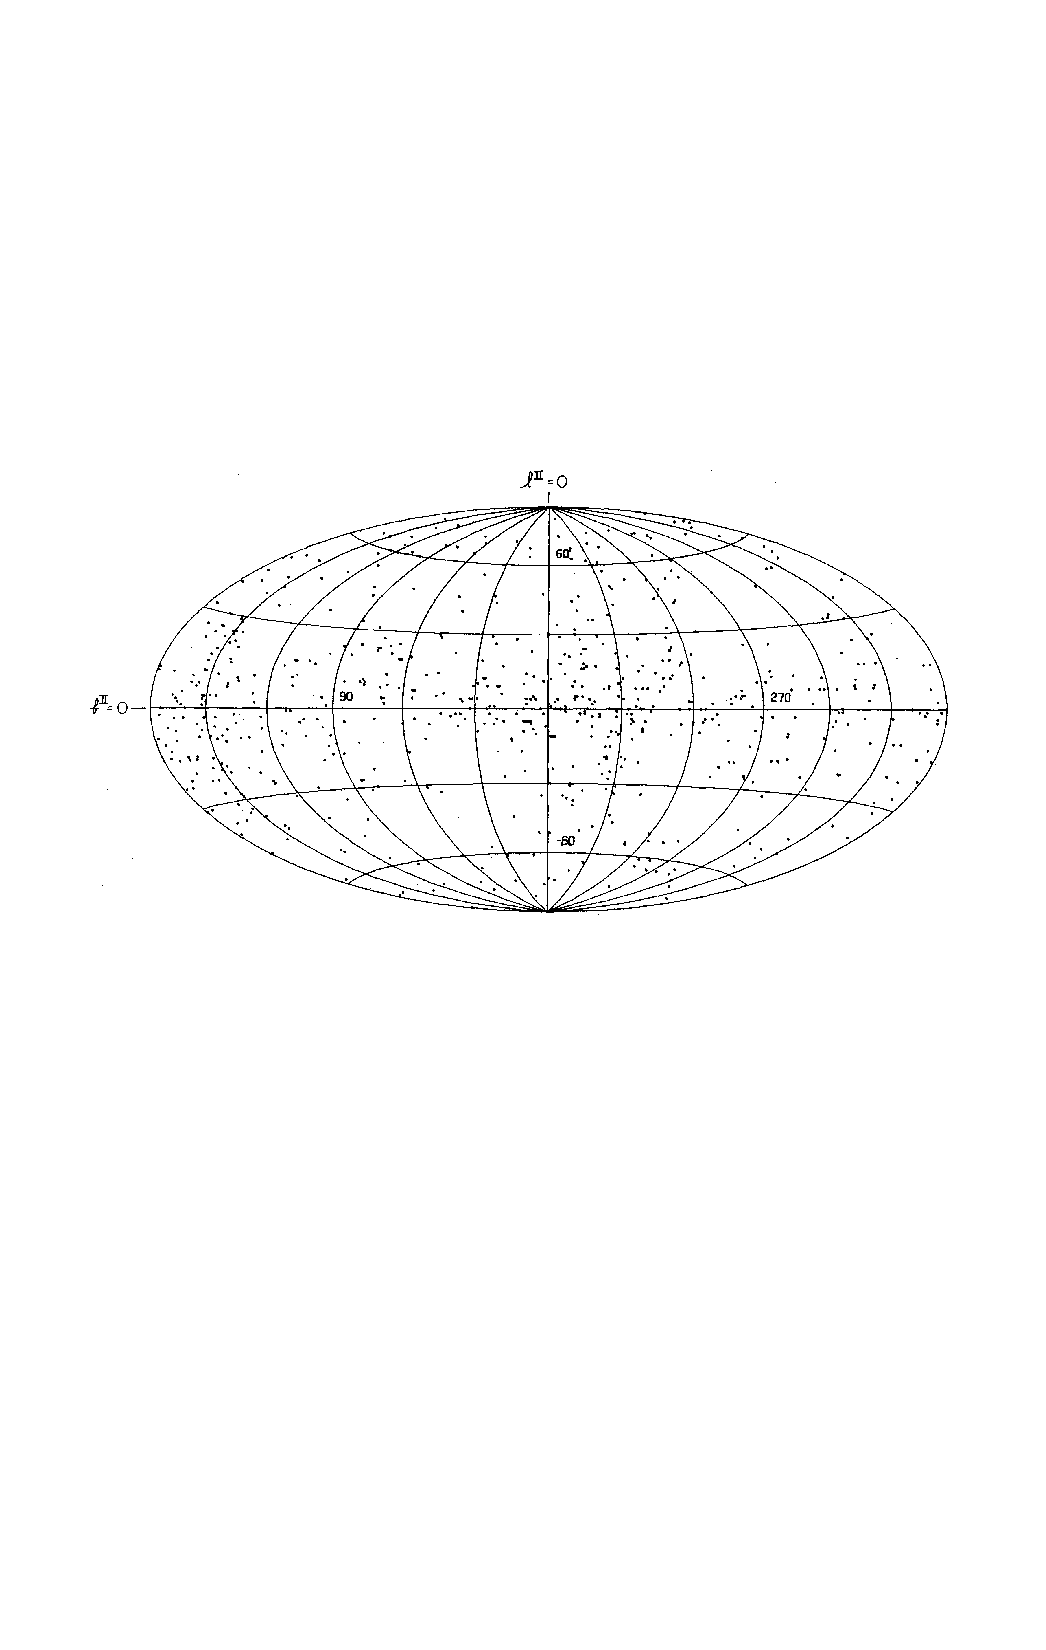
\includegraphics{chapters/introduction/figures/kraushaar_et_al_1972_skymap.pdf}
\figlabel{oso3_skymap}
\caption{The position of all 621 cosmic $\gamma$-rays
detected by \ac{OSO-3}. This figure is from 
\cite{kraushaar_1972_high-energy-cosmic}. }
\end{figure}

% ``The field of gamma-ray astronomy took great leaps forward'' -- wikipedia

  % ``Additional gamma-ray experiments flew on the OGO, OSO, Vela, and Russian
  % Cosmos series of satellites. However, the first satellite designed as a
  % ``dedicated'' gamma-ray mission was the second Small Astronomy Satellite
  % (SAS-2) in 1972.`` - http://imagine.gsfc.nasa.gov/docs/science/know_l1/history_gamma.html



The next major advancement in $\gamma$-ray astronomy came from
the \ac{SAS-2} and \cosb missions.

\ac{SAS-2} was a dedicated $\gamma$-ray detector
launched by \ac{NASA} in November 15, 1972.  \ac{SAS-2} was
\cite{fichtel_1975_high-energy-gamma-ray} It improved upon \ac{OSO-3}
by incorporating a spark chamber and having an overall larger size.
The size of the active area of the detector was 640 $\cm^2$ and the
experiment had a much improved effective area of $\sim 115\,cm^2$. The
spark chamber allowed for a seperate measurement of the electron and
positron tracks, which allowd for improved directional reconstruction
of the incident $\gamma$-ray. \ac{SAS-2} had a PSF $\sim5\degree$ at 30
\mev and $\sim1\degree$ at 1 \gev.

\ac{SAS-2} collected data for over 6 months before a power supply
failure ended data collection. \ac{SAS-2} Observed over 8,000
$\gamma$-ray photons covering $\sim55\%$ of
the sky including most of the Galactic plane.  
\ac{SAS-2} disovered strong emission
along the Galactic plane and particularly towards the Galactic
cente. It also discovered
pulsations from the
Crab \citep{fichtel_1975_high-energy-gamma-ray} and Vela pulsar
\citep{thompson_1977_sas-2-high-energy}.  In addition, \ac{SAS-2}
discovered Geminga, the first $\gamma$-ray source with no compelling
multiwavelenth counterpart \citep{thompson_1977_final-sas-2}. Gemina
was eventually discovered to be a pulsar by \ac{EGRET}
\citep{bertsch_1992_pulsed-high-energy} and retroactivly by \ac{SAS-2}
\citep{mattox_1992_observation-pulsed}.

% ``Cos-B was ESA's first satellite dedicated to a single experiment. Its
% scientific mission was to study in detail the sources of extra-terrestrial
% gamma radiation at energies above about 30 MeV. The originally foreseen
% duration of the mission was two years, but in fact Cos-B functioned
% successfully for 6 years and 8 months. During this time an extensive
% survey of the Galaxy was made in the energy range 50 MeV to 5 GeV.''
% -- http://sci.esa.int/science-e/www/area/index.cfm?fareaid=34

% ``Description Cos-B was the first ESA mission dedicated to the study of
% gamma-ray sources. Its results created a catalogue of these sources,
% known as the 2CG Catalogue, the first complete map of the gamma-ray
% emission from the disc of our Galaxy, the Milky Way, and the first
% detectable emission from an extra-galactic object 3C273.'' 
% -- http://www.esa.int/Our_Activities/Space_Science/Cos-B_factsheet

% cos b performance is described at:
%   http://www.rssd.esa.int/index.php?page=gr-tele&project=COSB

\cosb, an \ac{ESA} mission, was launched shortly after, on August
9, 1975.  Similar to \ac{SAS-2}, \cosb includd a spark chamber for
reading out the $\gamma$-ray events and had a peak effective area
of $\sim 50\,cm^2$ at $\sim400\,MeV$ It improved upon the design
\ac{SAS-2} by including a calorimiter below the spark chamber which
improved the energy resolution to $<100\%$ for energies $\sim 3\,\gev$
\citep{bignami_1975_cos-b-experiment}.

\cosb operated successfully for over 6 years and produced
the first detailed catalog of the $\gamma$-ray sky.
\ac{2CG} detailed the detection 25 $gamma$-ray sources
for $E>100\,\mev$ \citep{swanenburg_1981_second-catalog}.

\begin{figure}[htb]
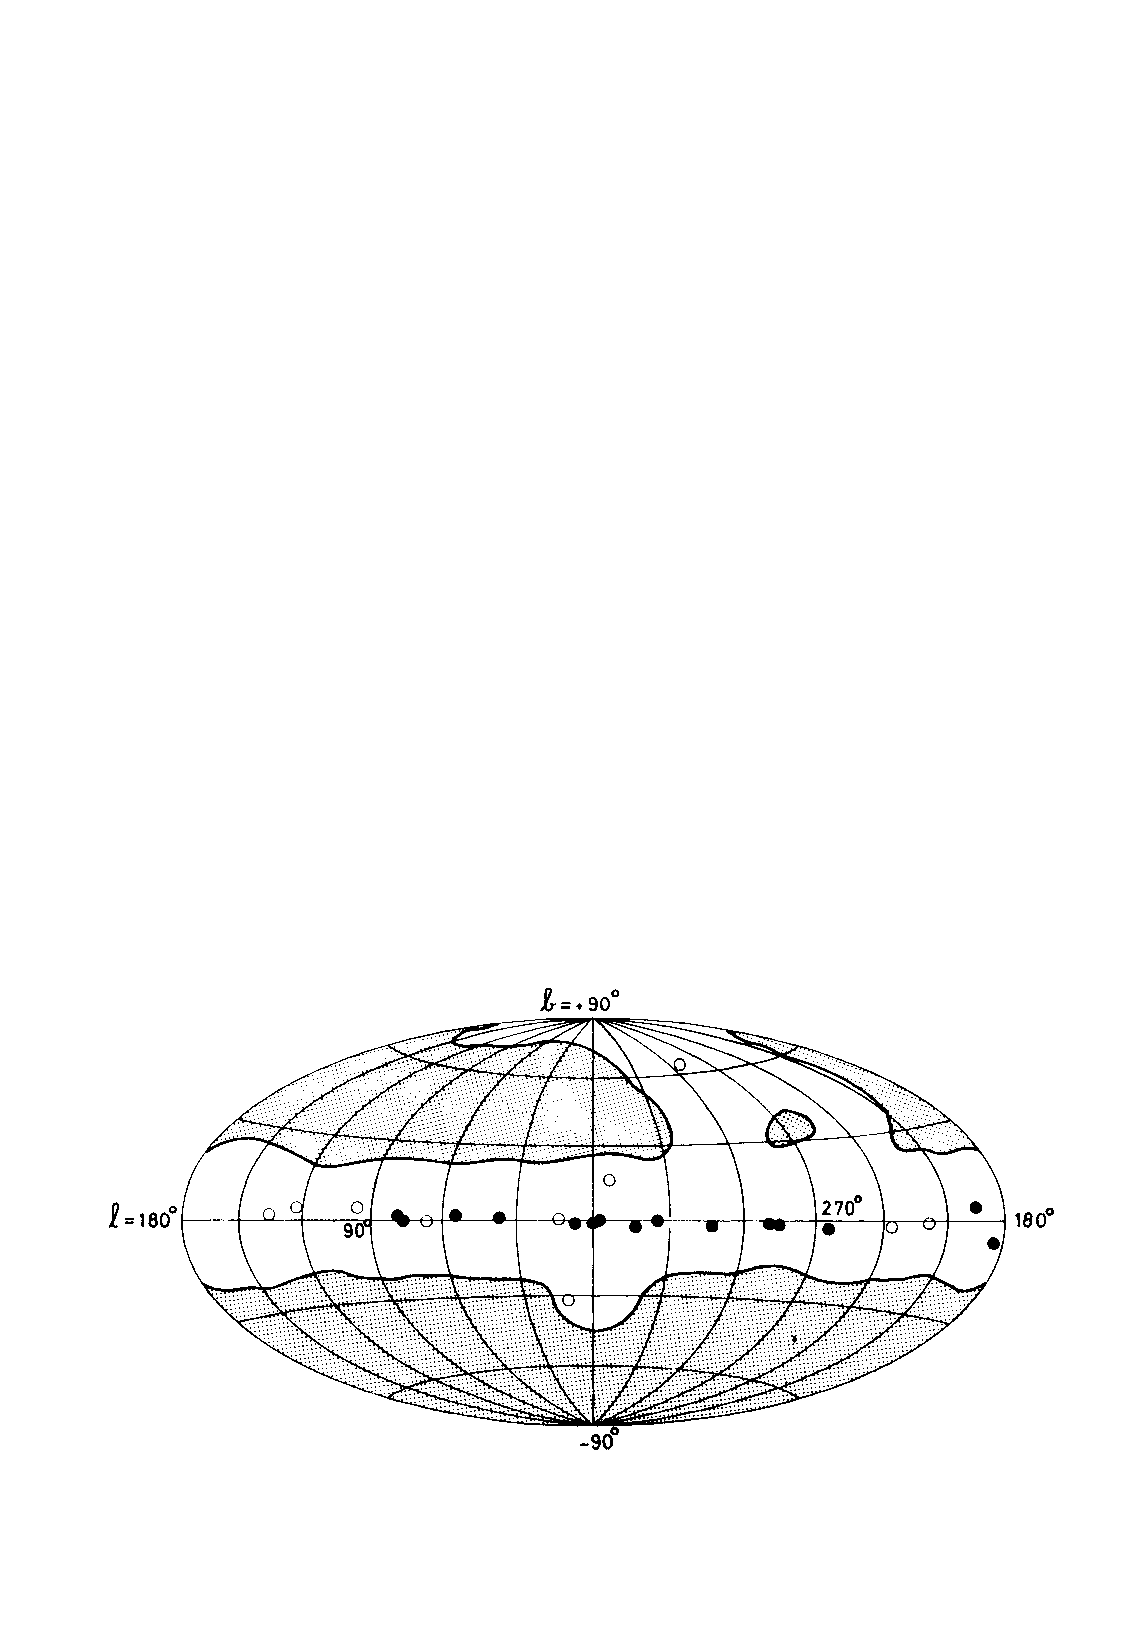
\includegraphics{chapters/introduction/figures/cos_b_2nd_catalog.pdf}
\figlabel{cos_b_skymap}
\caption{
The figure is from \cite{swanenburg_1981_second-catalog}.
}
\end{figure}


\todo[inline][3C27]

% 6 years and 8 months. During this time an extensive survey of the Galaxy was made in the energy range 50 MeV to 5 GeV.

: 2 Year catalog: 
\todo[inline]{Describe COS-B. What was its effective area}



\begin{itemize}
  \item EGRET
    % Good summary of EGRET Results:
    %  http://arxiv.org/pdf/0811.0738.pdf
  \item AGILE
  \item \todo[inline]{Short description of the history
    of TeV astronomy}
\end{itemize}





\section{The \fermi Gamma-ray Space Telescope}
\seclabel{fermi_telescope}

\begin{figure}[htbp]
  \centering
    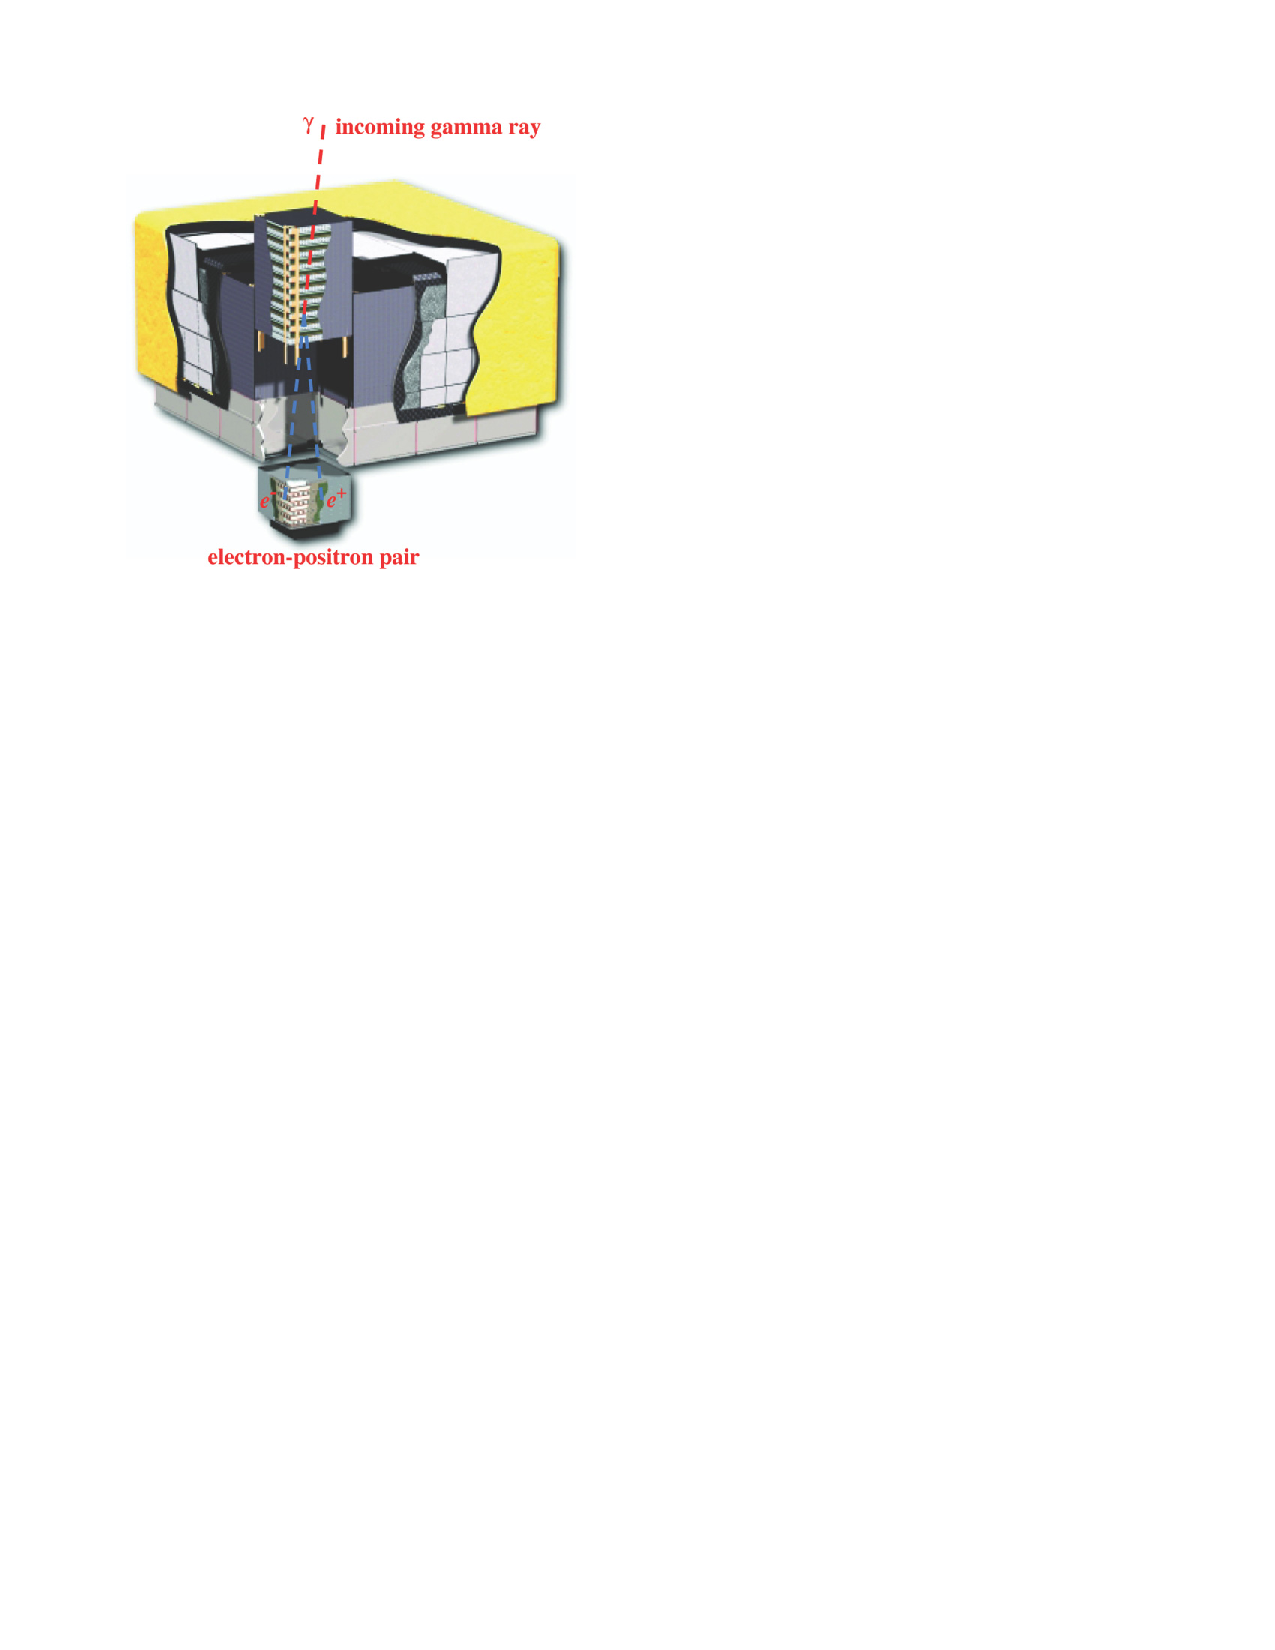
\includegraphics{chapters/introduction/figures/lat_detector_cutout.pdf}
  \caption{A schematic diagram of the \ac{LAT} with an incident $\gamma$-ray
    (red line) pair-converting into an electron and positron (blue lines)
    which are recorded in the tracker and calorimiter of the \ac{LAT}.
    This figure is taken from \citep{atwood_2009a_large-telescope}.  
    This diagram shows the three major subsystems of the \ac{LAT}:
    the tracker, the calorimiter, and the \ac{ACD}.
  }
  \figlabel{lat_detector_cutout}
\end{figure} 


The \fermi Gamma-ray Space telescope was launched on June 11, 2008 on
a Delta II heavy launch vehicle \citep{atwood_2009a_large-telescope}.
The primary since instrument on board \fermi is the \ac{LAT},
which is a pair-conversion telescope which detects $\gamma$-rays
in the energy range from $20\unitspace\mev$ to $>300\unitspace\gev$.
\figref{lat_detector_cutout} shows a schematic diagram of the \ac{LAT}.
With its unprecedent effective area and angular resolution, the \ac{LAT}
has drastically improved our understanding of the $\gamma$-ray sky.
In addition, \fermi contains the \Ac{GBM}, which is used to obseerve
\acp{GRB} in the energy range from $\sim8\unitspace\kev$ to $\sim40\unitspace\mev$.
See \cite{meegan_2009a_fermi-gamma-ray} for a description of the \ac{GBM}
detector.

\subsection{The \acs{LAT} Detector}

The \ac{LAT} is composed of three major subsystems: the tracker, the
calorimeter, and the \ac{ACD}. Fundamentally, the detector operates by
inducing an incident $\gamma$-ray to pair convert in the tracker into
an electron and positron pair. The electron and position travel through
the tracker and into the \ac{CsI} calorimiter.  The track they leave in
the tracker and the energy deposite they leave in the calorimter can be
used to infer the direction and energy of the incident $\gamma$-ray.

Both the tracker and calorimiter are $4\times4$ arrays, each composed of
16 modules.  Each tracker tower is divided into 18 tungsten converter
layers and 16 dual-silicon tracker planes ($x$ and $y$).  As a balance
between effective area and angular resolution, The top 12 tracker planes
have thin layers of tungsten which minimize the probability of secondary
scattering and improves the angular resolution of the \ac{LAT}, especially
for low-energy $\gamma$-rays. The bottom four tracker planes have layers
of tungsten $\sim6$ times thicker, which improves the likelihood of
conversion and therefore the effective area.  The ``front'' and ``back''
classificaiton for $\gamma$-rays refers to if they convert in the thin
or thick layers of the detector, respectivly.  Each calorimiter module
composed of eight layers of 12 \ac{CsI} crystals. The depth of the
calorimiter is 8.6 radiation lenghts adn the depth of entire insutrment
is 10.1 radiation lenths.

The \ac{ACD}, the third subsystem on the \ac{LAT}, provides provides
background rejection by of the charged particle background incident
on the \ac{LAT}.  The \ac{ACD} surrounds the tracker and is composed
of 89 plastic scintillator tiles ($5\times5$ on the top and 16
on each of the sides). The \ac{ACD} has a 0.9997 efficiency for
detcting singly-charged particles entering the \ac{LAT}.  A detailed
discussion of the various subsystems of the LAT can be found in
\citep{atwood_2009a_large-telescope}.

\subsection{Performance of the \acs{LAT}}

The \ac{LAT} 
has an unprecidended effective area ($\sim9,500\unitspace\cm^2$),
single-photon energy resolution ($\sim10\%$), and single-photon
angular resolution ($\sim3\fdg5$ at $\energy=100\unitspace\mev$
and decreasing to $\lesssim0\fdg15$ for $\energy>10\unitspace\gev$)
\citep{atwood_2009a_large-telescope}.

With its $2.4\unitspace\steradian$ filed of view,

\todo[inline]{forward reference description of analysis of LAT data}


\section{Astrophysical Sources of Gamma-rays}
\seclabel{astrophysical_sources}

\subsection{Pulsars}

``The gravitational collapse of the core of a massive star into a neutron
star (e.g., Baade \& Zwicky 1934) releases enough energy to power a
supernova explosion (e.g., Zwicky 1938).'' -- gelfand\_2009\_dynamical-model

``First widely accepted prediction of an ultra-dense star
was given by Zwicky and Baade (1934). Proposed the idea that
a supernova represents the transition of an ordinary star
into a neutron star, consisting mainly of neutrons.'' --
\url{http://www.atnf.csiro.au/research/pulsar/orange10/pdf/RaiYuenOrange2010.pdf}

% good details from "Pulsar Astronomy" By Andrew G. Lyne, Francis Graham-Smith

Pulsars were first discovered in 1967 by Jocelyn Bell Burnell and Antony
Hewish \citep{hewish_1968_observation-rapidly}. They had constructed a
radio telescope that used interplanetary scintillation wiht the intention
of observing quasars.  In the process, they detected a source with a
periodicity of 1.3 \second.

\todo[inline]{Make note of ``Air force had early warning of pulsars'' paper}

Even before the discovery, \cite{pacini_1967_energy-emission} had predicted
the existence of \acp{NS}.  Shortly following the 1967 discovery,
\cite{gold_1968_rotating-neutron} and \cite{pacini_1968_rotating-neutron}
argued that the observed pulsar was a rotating \ac{NS}.

The discovery of many more pulsars came quickly.  In 1968, and the
Vela pulsar \citep{large_1968_pulsar-supernova} and the Crab pulsar
\citep{staelin_1968_pulsating-radio} were discovered.

% Info came from the book ``Pulsar Astronomy'' by Lyne.
The first pulsar observed at optical frequencies was the
Crab, discovered in 1969 shortly after its radio discvoery
\citep{cocke_1969_discovery-optical}.
In the same year, the first X-ray pulsations were discovered from
the same source. At the time, there were no space-based X-ray
observatories, so observations had to be performed from rockets.
The discovery was carried out almost concurrently by a group
at \gls{NRL} \citep{fritz_1969_x-ray-pulsar} and at \gls{MIT}
\citep{bradt_1969_x-ray-optical}.  Using proportional counters,
these experiments showed that the pulsed emission from 
the Crab extended to X-ray energies and that, for this source,
the X-rays emission was a factor $>100$ more energetic than
the observed visible emission.

\begin{itemize}
  \item I read somewhere, but don't have the reference (it was one
    of htose verbose history books on pulsars), that originally
    the neutron star hypothesis wasn't well accepted. But then
    one pulsar was found with a very short period (I think the Crab)
    which, for causaility reasons, had to be small enough taht it
    seemed to confirm the Neutron star hypotehsis.
  \item For Crab describe spin down?: ``and these pulsations were then shown to be slowing down at a
    rate of 36 ns per day (Richards \& Comella 1969).'' -- \cite{gaensler_2006_evolution-structure}
\end{itemize}

As was discussed in \secref{history_gamma_ray_detectors},
$\gamma$-ray emission from the Crab was detected only 2 years
later \citep{browning_1971_detection-pulsed}.

\todo{First gamma-ray detection}

ATNF catalog?

\begin{itemize}
  \item ``There are currently more than 1,800 pulsars in the ATNF on-line
  catalog [Manchester et al., 2005], with rotation periods in the rage
  0.0016-12 seconds (Figure 3.1) and derived spin down
  luminosities in the range XXX - XXX erg/s.'' -- dalton\_2011\_identication-gamma-ray
\end{itemize}

EGRET pulsars?

The state of the art in $\gamma$-ray detection of pulsars
will be included in an upcomming pulbication.
2PC: \secref{second_pulsar_catalog}

\todo[inline]{When was the PSR, PWN connection made}


\subsection{\Acptitle{PWN}}

% Good history of observations of crab nebulae:
%  * chapter 1 of "The Crab Nebula" by Rodney Deane Davies

% Good history paper: ``Pulsar Wind Nebulae:
%   On their growing diversity and association
%   with highly magnetized neutron stars''
%   by Samar Safi-Harb
%   -- http://arxiv.org/pdf/1211.0852.pdf

% Good paper on Crab Nebula: ``{The Crab Nebula: An Astrophysical Chimera}'' by
%   J. Jeff Hester

% Good review of PWN: 
%   ``The Evolution and Structure of Pulsar Wind Nebulae''
%   Bryan M. Gaensler and Patrick O. Slane

% Good review of PWN:
%  ``{Pulsar Wind Nebulae in the Chandra Era}''
%  O. Kargaltsev and G. G. Pavlov


% lots of INFO on M1 (crab): http://messier.seds.org/m/m001.html


A \gls{PWN} is a diffuse nebula of shocked relativistic particles.
A \glspl{PWN} surrounds and is powered by an accompanying pulsar. 
\glspl{PWN} have been observed long before the discovery of pulsars, but
the pulsar/\gls{PWN} connection could not be made until
after the detection of pulsars.

The most famous \glspl{PWN} is the Crab nebula, associated with
the Crab pulsar.

\begin{itemize}
  \item Chinese SN observations of Crab Nebulae: (p128 of ``The Crab Nebula: An Astrophysical Chimera'')
     ``It was probably also recorded by Anasazi Indian artists (in
     present-day Arizona and New Mexico), as findings in Navaho Canyon and
     White Mesa (both Arizona) as well as in the Chaco Canyon National
     Park (New Mexico) indicate; there's a review of the research on
     the Chaco Canyon Anasazi art online. In addition, Ralph R. Robbins
     of the University of Texas has found Mimbres Indian art from New
     Mexico, possibly depicting the supernova.'' -- http://messier.seds.org/m/m001.html
\end{itemize}

It was discovered in
1731 by physician and amateur astronomer John Bevis.  This source was
going to be published in his sky atlas {\em Uranographia Britannica}, but
the work was never publisehd because his published filed for bankrupcy
in 1950.  Figure~\figref{bevis_crab} shows Beavis' plate containing
the Crab nebula.  A detailed history of John Bevis' work can be found
in \cite{ashworth_1981_bevis-uranographia}.


\begin{figure}[htb]
  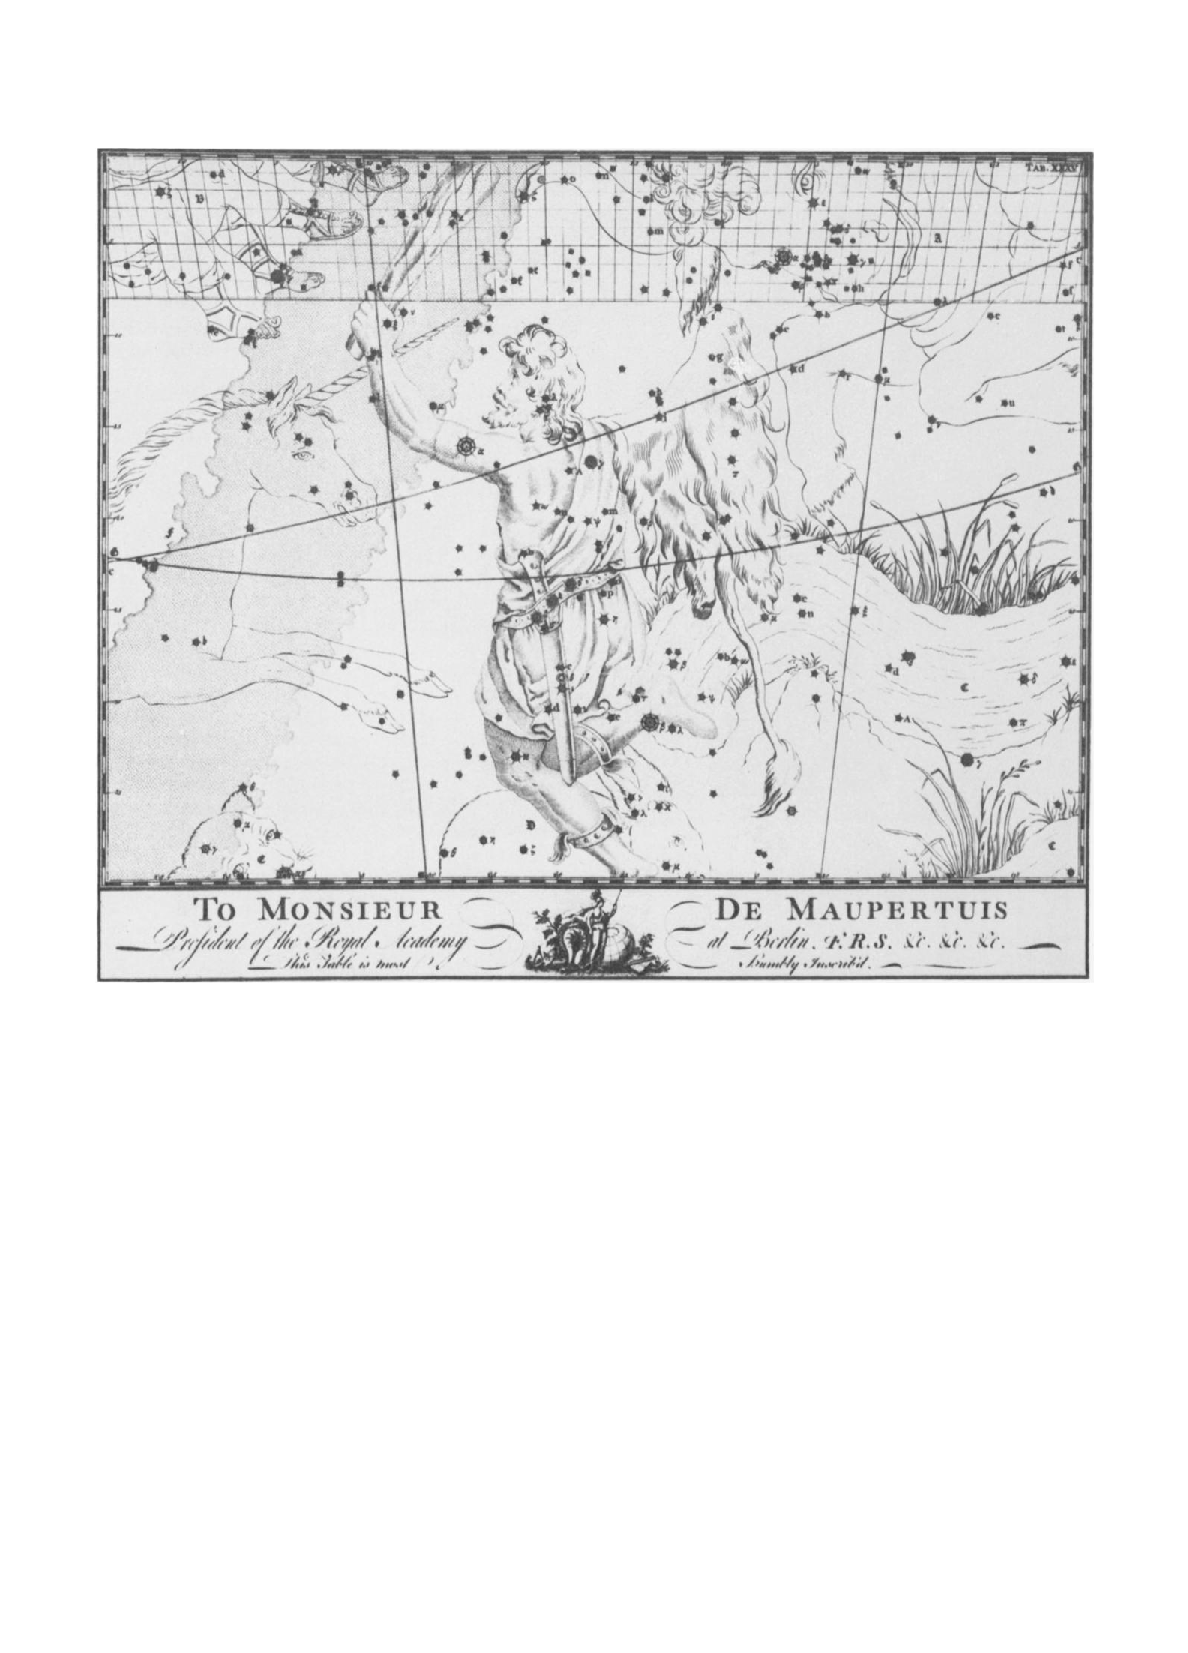
\includegraphics[width=\textwidth]{chapters/introduction/figures/bevis_crab.pdf}
  \figlabel{bevis_crab}
  \caption{The Orion plate from Bevis' book {\em Uranographia Britannica}.
  The Crab nebula can be found on the horn of Taurus the Bull 
  on the top of the figure and the source is marked by a 
  cloudy symbol.
  This figure was reproduced from \cite{ashworth_1981_bevis-uranographia}.}
\end{figure}

\begin{itemize}
  \item Crab Nebulae is M1 in Charles Messier's catalog 1758 
    (p128 of ``The Crab Nebula: An Astrophysical Chimera'')
  \item Connection to 1054:
    ``Lundmark (1921) suggested a connection between the Crab Nebula and the event of 1054 AD''
    (p128 of ``The Crab Nebula: An Astrophysical Chimera'')
    ``The Crab Nebula (Fig. 1) is almost certainly associated with a
    supernova (SN) ex- plosion observed in 1054 CE (Stephenson \& Green
    2002, and references therein).'' -- ``The Evolution and Structure of Pulsar Wind Nebulae'' 
    Bryan M. Gaensler and Patrick O. Slane
  \item ``The same year, J.C. Duncan of Mt. Wilson Observatory compared
    photographic plates taken 11.5 years apart, and found that the
    Crab Nebula was expanding at an average of about 0.2'' per year;
    backtracing of this motion showed that this expansion must have
    begun about 900 years ago (Duncan 1921). Also the same year, Knut
    Lundmark noted the proximity of the nebula to the 1054 supernova
    (Lundmark 1921).`` -- http://messier.seds.org/m/m001.html
    ``In 1942, based on investigations with the 100-inch Hooker telescope
    on Mt. Wilson, Walter Baade computed a more acurate figure of 760
    years age from the expansion, which yields a starting date around
    1180 (Baade 1942); later investigations improved this value to about
    1140. The actual 1054 occurrance of the supernova shows that the
    expansion must have been accelerated.'' -- http://messier.seds.org/m/m001.html
  \item ``but it was not until 1942 that Duyvendak (1942) and Mayall \&
  Oort (1942) presented complete studies of modern observations of the
  expanding nebula and of the early Chinese records. It was this work
  that established unambiguously that the Crab is the remnant of SN1054.''
    (p128 of ``The Crab Nebula: An Astrophysical Chimera'')
  \item ``1949, the Crab nebula was identified as a strong source
  of radio radiation (Bolton et.al. 1949), discovered 1948 named
  and listed as Taurus A (Bolton 1948), and later as 3C 144.'' -
  http://messier.seds.org/m/m001.html




  \item Synchrotron emission hypotehsis: ``while the inner, blueish
      nebula emits continuous light consisting of highly polarised so-called
      synchrotron radiation, which is emitted by high-energy (fast moving)
      electrons in a strong magnetic field. This explanation was first
      proposed by the Soviet astronomer J. Shklovsky (1953) and supported
      by observations of Jan H. Oort and T. Walraven (1956).'' -- http://messier.seds.org/m/m001.html
  \item ``X-rays from this object were detected in April 1963 with a
      high-altitude rocket of type Aerobee with an X-ray detector developed
      at the Naval Research Laboratory; the X-ray source was named Taurus
      X-1. Measurements during lunar occultations of the Crab Nebula on
      July 5, 1964, and repeated in 1974 and 1975, demonstrated that the
      X-rays come from a region at least 2 arc minutes in size, and the
      energy emitted in X-rays by the Crab nebula is about 100 times more
      than that emitted in the visual light''
        -- http://messier.seds.org/m/m001.html
  \item Association of Crab pulsar with Crab nebulae were 
    discussed in \citep{staelin_1968_pulsating-radio}.

\item
"Just after discovery of pulsars, Gunn \& Ostriker (1969) suggested
that particles can be accelerated to very high energies in the pulsar
wind zone." -- "Relativistic Astrophysics and Cosmology" by Shapiro


  \item TEV observations of Crab. brightest soruce in the sky\ldots
  \item Now many radio, x-ray PWNe. Count form PWN catalog: http://www.physics.mcgill.ca/~pulsar/pwncat.html
    ``Observations over the last several decades have identified 40 to 50
    further sources, in both our own Galaxy and in the Magellanic Clouds,
    with properties similar to those of the Crab Nebula (Green 2004;
    Kaspi, Roberts \& Harding 2006)'' -- \cite{gaensler_2006_evolution-structure}
  \item How many TeV PWNe in TeVCat? http://tevcat.uchicago.edu/ (31 by my preliminary count)
\end{itemize}






\section{Radiation Processes in Gamma-ray Astrophysics}

Nontermal radiation observed from astrophysical sources
is typically believed to originate in syncrotron
\ac{IC}, and the decay of neutral \pion particles.

\subsection{Synchrotron}


\begin{figure}[htbp]
  \centering 
    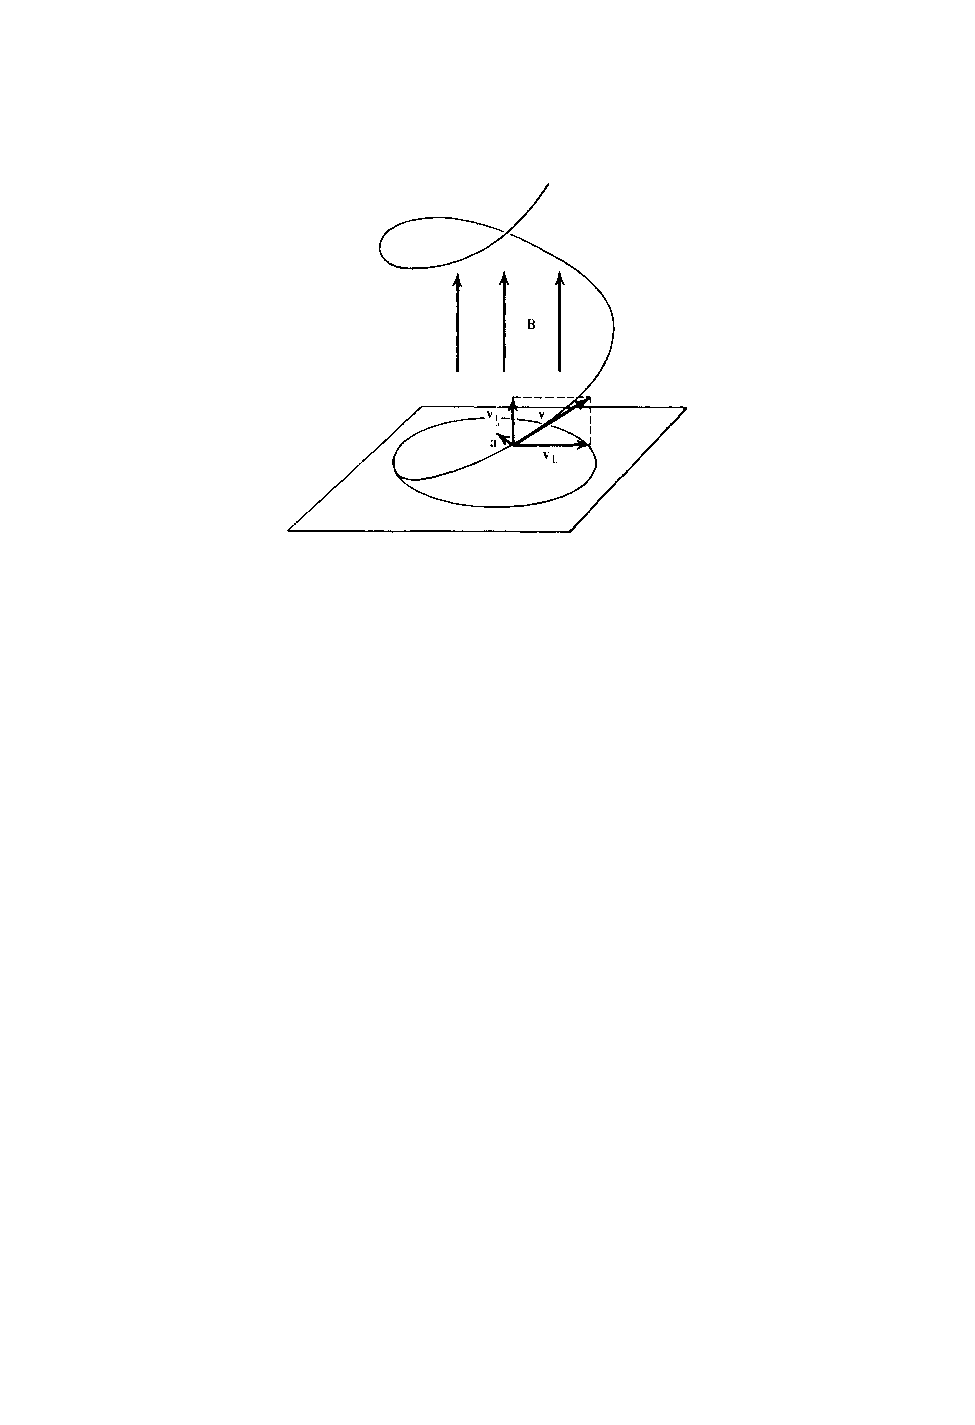
\includegraphics{chapters/introduction/figures/syncrotron_radiation_spiral.pdf}
    \caption{In synchrotron radiation, charged particles spiral along
      magnetic filed lines, radiating photons as they accelerate.}
  \figlabel{syncrotron_radiation_spiral}
\end{figure}


The synchrotron radiation processes is commonly observed in
astrophysics. It is caused when charged particles, typically
electrons, spiral around magnetic field lines.  As they
accelerate, they radiate photons.  This process is illustrated in
\figref{syncrotron_radiation_spiral}.
This emission is discussed thoroughly in
\cite{blumenthal_1970a_bremsstrahlung-synchrotron} and
\cite{rybicki_1979a_radiative-processes}.
In what follows, we adopt the notation from
\cite{houck_2006a_models-nonthermal}.

A charged particle of 
mass $\mass$ and charge $\charge$ in a magnetic field
of strength 
\MagneticFieldVector
will experince an
electromagnetic force:
\begin{align}
% equation 6.1a in R&L 1979
  \dbydt (\gamma m \VelocityVector) = & \frac{q}{c} \cross{\VelocityVector}{\MagneticFieldVector}
\end{align}
This force will cause a particle to accelerate around
the magnetic field lines, causing it
to radiate by maxwell's equations.

The power emitted at a frequency $\frequency$ 
by particle spiraling will be
\begin{equation}
% equation 6.33 in R&L 1979
  \eqnlabel{power_emitted_particle_sync}
  \power_\text{emitted}(\frequency) = 
  \frac{\sqrt{3} \charge^3 B \sin\alpha}{\mass \speedoflight^2} F(\frequency/\frequency_c)
\end{equation}
where $\alpha$ is the angle between the particle's velocity vector and
magnetic field vector.
Here,
% equation 6.31c in R&L 1979
\begin{equation}
  F(x) \equiv x \int_x^\infty K_{\tfrac{5}{3}} (\xi) d\xi,
\end{equation}
and
\begin{equation}
% equation 6.11a in R&L 1979
\frequency_c = \frac{3q \MagneticField \gamma^2}{4\pi \mass \speedoflight} 
\sin\alpha \equiv \nu_0 \gamma^2 \sin\alpha
\end{equation}

Because power is inversely-proportional to mass, synchotron radiation
is almost always assumed to come from electrons.

Now, we assume a population of particles and compute the total
emission. We say that $\ParticleDistribution(\momentum,\alpha)$ is the number of particles
per unit momentum and solid angle with a momentum $\momentum$ and
pitch angle $\alpha$.

We find the total power emitted by integrating over particle
momentum and distribution
\begin{equation}
  \frac{\derivative W}{\derivative\time}=
  \int \derivative \momentum 
  \int \derivative \solidangle
  \power_\text{emitted}(\frequency)
  \ParticleDistribution(\momentum,\alpha)
\end{equation}
If we assume the pitch angles of the particles to be isotropically
distributed and include \eqnref{power_emitted_particle_sync}, we
find that the photon emission per unit energy and time is
\begin{equation}
  \frac{\derivative \ParticleDistribution}{\derivative \omega \derivative \time} =
  \frac{\sqrt{3}q^3 B}{h m_e c^2 \angularfrequency}
  \int \derivative\momentum
  \ParticleDistribution(\momentum)
  R \left(\frac{\omega}{\omega_0 \gamma^2}\right)
\end{equation}
where
\begin{equation}
  R(x) \equiv \frac{1}{2} \int_0^\pi
  \derivative \alpha \sin^2 \alpha
  F\left(\frac{x}{\sin\alpha}\right)
\end{equation}

It is typical in astrophysics to assume a 
a power-law distribution of electrons written as
\begin{equation}
% equation 6.20a in R&L 1979
\eqnlabel{ElectronPowerLawEnergyDistribution}
  \ParticleDistribution(\momentum) \derivative\momentum = 
  \kappa \momentum^{-\spectralindex} \derivative\momentum.
\end{equation}
For a powerlaw distribution of photons integrated over
pitch angle, we find
\begin{equation}
\TotalPower(\angularfrequency) \propto \kappa \MagneticField^{(p+1)/2} 
\angularfrequency^{-(p-1)/2}.
\end{equation}
See, \cite{rybicki_1979a_radiative-processes} 
or \cite{longair_2013a_energy-astrophysics} for a full derivation.
This shows that, assuming a power-law electron distribution,
the electron spectral index can be related to the photon spectral
index.

\subsection{\Actitle{IC}}

Normal compoton scattering involves a photon colliding with a free electron
and transfering energy to it. In \ac{IC} scattering, a high-energy 
electron interacts with a low-energy photon imparting energy to it.
This process occurs when highly-energetic electrons interact with
a dense photon field.

The derivation of \Ac{IC} emission requires a quantum
electrodynamical treatment. It was first computed in
\cite{klein_1929a_streuung-strahlung}, and the derivation is described
in \cite{blumenthal_1970a_bremsstrahlung-synchrotron}.  In what follows, we follow
the notational convetion of \cite{houck_2006a_models-nonthermal}.

We assume a population of relativistic ($\gamma\gg1$) electrons
written as $\ParticleDistribution(\momentum)$ which is contained inside isotropic 
photon distribution with number density $n(\omega_i)$.

The distribution of photons 
emitted by \ac{IC} scatter is
written as
\begin{equation}
  \frac{\derivative\ParticleDistribution}{\derivative\omega\derivative\time} = 
  c \int d \omega_i n(\omega_i)
  \int_{p_\text{min}}^\infty  dp
  \ParticleDistribution(p) 
 \KleinNishinaCrossSection(\gamma,\omega_i,\omega)
\end{equation}
where $\omega$ is the outgoing photon energy written
in units of the electron rest mass energy, $\omega\equiv h\nu/(m_e c^2)$,
and $\KleinNishinaCrossSection$ is the Klein-Nishina cross section.

The Klein-Nishina cross section is
\begin{equation}
\KleinNishinaCrossSection(\gamma,\omega_i,\omega) = \frac{2\pi r_0^2}{\omega_i \gamma^2}
  \left[
  1 + q - 2q^2 + 2q\ln q + \frac{\tau^2 q^2 (1-q)}{2(1+\tau q)}
  \right]
\end{equation}
Here,
\begin{equation}
  q \equiv \frac{\omega}{4 \omega_i \gamma (\gamma-\omega)},
\end{equation}
$\tau \equiv 4\omega_i \gamma$, and $r_0 = e^2/(m_e c^2)$ is the classical
electron radius.
The threshold electron lorentz factor is
\begin{equation}
  \gamma_\text{min} =
  \frac{1}{2} 
  \left(
  \omega + \sqrt{\omega^2 + \frac{\omega}{\omega_i}}
  \right)
\end{equation}

Typically, \ac{IC} emision is assumed to originate when
a power-law distribution of electrons
(see \eqnref{ElectronPowerLawEnergyDistribution})
interacts with
a thermal photon distribution
\begin{equation}
  n(\omega_i) = 
  \frac{1}{\pi^2\lambda^3} 
  \frac{\omega_i^2}{e^{\omega_i/\Theta} -1}
\end{equation}
where $\lambda=\hbar/(m_e c)$ and $\Theta=kT/(m_e c^2)$.
Typically, \ac{IC} emission happens off CMB photons
with $T=2.725\unitspace\kelvin$.
We conclude by noting that the free-parameters of 
\ac{IC} emission are the the assumed particle spectrum
and photon field.

\subsection{Bremsstrahlung}

Bremsstrahlung radiation is compoosed of electron-electron and electron-ion interactions.
In either case, 
we assume a 
differential spectrum of accelerated electrons $\ParticleDistribution_\electron(\energy)$ 
that interacts with a target density of electrons (\ElectronDensity) or ions (\IonDensity).

\begin{equation}
  \frac{\derivative \ParticleDistribution}{\derivative\energy\derivative\time} =
  \ElectronDensity \int \derivative\energy
  \ParticleDistribution_\electron(\energy) \velocity_\electron
  \frac{\derivative\CrossSection_{\electron\electron}}{\derivative\energy} +
  \IonDensity \int \denergy
  \ParticleDistribution_\electron(\energy) \velocity_\electron
  \frac{\derivative\CrossSection_{\electron\AtomicNumber}}{\derivative\energy}
\end{equation}

Here, $\velocity_\electron$ is the velocity of the
electron, and $\CrossSection_{\electron\electron}$ and
$\CrossSection_{\electron\AtomicNumber}$ are the electron-electron and
electron-ion cross sections.
The actual formulas for 
$\derivative\CrossSection_{\electron\electron}/\derivative\energy$
and 
$\derivative\CrossSection_{\electron\AtomicNumber}/\derivative\energy$
are quite involved.  The electron-electron cross section was worked out
in \cite{haug_1975a_bremsstrahlung-production}.  The electron-ion cross
section is called the The Bethe-Heitler cross-section and is worked
out in the Born approximation in \cite{heitler_1953a_quantum-theory}
and \cite{koch_1959a_bremsstrahlung-cross-section}.  A more
accurate relativisatic correction to this formula is given in
\cite{haug_1997a_nonrelativistic-bremsstrahlung}.  We refer
to \cite{houck_2006a_models-nonthermal} for a detailed numerical
implementation of these formulas.

\subsection{Pion Decay}

Neutral \pion decay occurs when highly-energetic protons interact with
thermal protons. This
emission happens when protons decay into neutral pions through $pp \processarrow
\pion + X$ and the $\pion$ subsequently decay through $\pion \processarrow 2\gamma$.
The gamma-ray emission from neutral pion decay can be computed
as
\begin{equation}
  \frac{\derivative\ParticleDistribution}{\derivative\energy\derivative\time} = 
  \HydrogenDensity \int \denergy \velocity_\proton \ParticleDistribution_\proton(\energy) 
  \frac{\derivative\CrossSection_{\proton\proton}}{\derivative\energy}
\end{equation}
Here, $\ParticleDistribution_\proton(\energy)$
is the differential proton distribution,
$\derivative\CrossSection_{\proton\proton}/\derivative\energy$
is $\gamma$-ray cross section through proton-proton interactions, and
$\HydrogenDensity$ is the target hydrogen density.  The computation
of $\derivative\CrossSection_{\proton\proton}/\derivative\energy$ is
rather invovled. Typically, people employ a parmaeteriztaion of 
a very detaield calcuation of the cross section 
from \cite{kamae_2006a_parameterization-gamma}.


\section{The Pulsar/\glslink{PWN}{Pulsar Wind Nebulae} System}

Describe pulsar/PWN/SNR system:

\begin{itemize}
  \item Describe how a supernova creates an SNR and leaves behinda
    a pulsar wind nebula. 
  \item ``Pulsars are now known to be created in Supernova events,
    where the dense stellar core created in thermonuclear reactions is
    left over after the nova event. Depending on its mass, the remaining
    solar core may form a neutron star or a black hole. The determining
    criterion is the Chandrasekhar limit (MCh) given by:'' -- dalton\_2011\_identication-gamma-ray
\end{itemize}

\subsection{Pulsar Properties}

\todo[inline]{XXXXXXXXXXXXXXXX}

% Good discussion of PWN physics with some simple formulas: 
%   ``The Evolution and Structure of Pulsar Wind Nebulae''
%   Bryan M. Gaensler and Patrick O. Slane


% good discussion of radius of termination shock in: kargaltsev_2008_pulsar-nebulae

% Another review paper (looks to describe pulsar modeling):
%  ``High Energy Studies of Pulsar Wind Nebulae''
%     Patrick Slane

% Also, Adam Van Etten's thesis: 1.1 Pulsar Wind Nebula Structure

% Good reference: ``Carroll and Ostlie'' page 593

% good refernce on PWN physics: \cite{fuste_2007_g-ray-observations}

\begin{itemize}
  \item ``Following this discovery, a theoretical understanding was
  soon developed in which the central pulsar generates a magnetized
  particle wind, whose ultrarelativistic electrons and positrons radiate
  synchrotron emission across the electromagnetic spectrum (Pacini \&
  Salvati 1973, Rees \& Gunn 1974). The pulsar has steadily released
  about a third of its total reservoir of ???? ergs
  of rotational energy into its surrounding nebula over the last 950
  years. This is in sharp contrast to shell-like SNRs, in which the
  dominant energy source is the ??? ergs of kinetic energy
  released at the moment of the original SN explosion.''  -- \cite{gaensler_2006_evolution-structure}
  \item 
    % described in Adam Van Etten's thesis
    What is terminaltion shock of PWNe.
  \item 
    How is pulsar outflow accelerated at shock?
\end{itemize}


\todo[inline]{Find a plot of a rotating pulsar. The simplest
rotating dipole model}

The energy powering pulsars and \glspl{PWN} is comonly
believed to originate in rotational kintetic energy stored in
the netutron star. 
Both the period \period and the period derivative
$\perioddot=d\period/d\time$ can be directly observed for a pulsar
and typically the pulsar is slowing down (\perioddot<0).
We write the rotational kinetic energy as
\begin{equation}
  \energyrotational = \tfrac{1}{2} I \angularfrequency^2
\end{equation}
where $\omega = 2\pi/\period$ and \period is the period of
rotation of the pulsar. We make the conection between
the pulsar's spin-down energy and the rotational kintecit energy as
$\energydot = - \derivative\energyrotational/\dtime$

The rotational kinetic energy in a pulsar can be written as
\begin{equation}
  \energydot = 4\pi^2 \momentofinertia \perioddot/\period^2,
\end{equation}
where \momentofinertia is the moment of inertia.
For a uniform sphwere,
\begin{equation}
  \momentofinertia = \frac{2}{5} M R^2
\end{equation}
Pulsars are assumed to be uniform spheres with $R=10\unitspace\km$
and $M=1.4\solarmass$, which leads to a canonical moment of inertia of
$\momentofinertia=10^{45}\unitspace\gram\cm^{-2}$.

It is believed that as the pulsar spins down, the this rotational energy
is released as pulsed electromagnetic radiation and also as a wind of
electrons and positrons accelerated in the magnetic field of the pulsar.

As the pulsar slows down, it released the rotational kinetic energy
\begin{equation}
  \energydot = - \frac{4 \pi^2 \momentofinertia \perioddot}{\period^3}
\end{equation}
where \perioddot is the rate of decrease in the period of the pulsar.

\todo[inline]{Discuss uniform dipole model}

We conventionally assume that the period and period derivative are related
by the equation
\begin{equation}\eqnlabel{angular_frequency_derivative_relation}
  \angularfrequencydot \propto \angularfrequency^\breakingindex
\end{equation}
where $\angularfrequency=2\pi/\period$, and $\breakingindex$
is the pulsar breaking index. 

\begin{itemize}
  \item ``though n has only been confidently measured for five pulsars,
  in each case falling in the range 2 < n < 3 (Livingstone et al. (2007)
  and references therein).'' -- Adam Van Etten's thesis
\item ``The braking index is the power to which the slowdown in angular
velocity occurs, and is defined as:
  \begin{equation}
    n = \frac{\period \perioddotdot}{\perioddot} + 2
  \end{equation}
  '' -- keogh\_2010\_search-pulsar
\end{itemize}

Equation \eqnref{angular_frequency_derivative_relation} is
a Bernoulli differential equation which can be integrated to solve for time

\begin{equation}
  T = \frac{\period}{(\breakingindex-1) |\perioddot|}
  \left(
  1-\left(\frac{\period_0}{\period}\right)^{(\breakingindex-1)}
  \right)
\end{equation}

\begin{itemize}
  \item TODO: cite Manchester \& Taylor 1977
\end{itemize}



\begin{equation}
  \pulsarage = \period/2\perioddot
\end{equation}


\begin{itemize}
  \item What is a typical moment of inertia, typical dE/dT
  \item What fraction of pulsar energy is released observationally
\end{itemize}

\subsection{Pulsar Magnetosphere}

\subsection{Pulsar Wind Nebulae}

\begin{itemize}
  \item Discuss termination shock (i.e. section 3.3.2 of dalton\_2011\_identication-gamma-ray
  \item The radius of the termination shock is
    \begin{equation}
      \radiusterminationshock = \sqrt{\frac{\energydot}{\tfrac{4}{3}\pi \pressureISM \speedoflight}}
    \end{equation}

\end{itemize}

\todo[inline]{Discuss pulsar evolution ``The Evolution and Structure of
Pulsar Wind Nebulae'' -- Bryan M. Gaensler and Patrick O. Slane}

\todo[inline]{Describe Mattana's work on PWNe: ``On the evolution of
the Gamma- and X-ray luminosities of Pulsar Wind Nebulae''}




\section{Modeling the Galactic Diffuse and Isotropic Gamma-ray Background}
\seclabel{modeling_background}

\todo[inline]{Include discussion of modeling, if time permitting}

\begin{itemize}
  \item Discuss the historical Observations of galactic diffuse emission

    Mention how \gls{OSO-3} first detected the $gamma$-rays from the galaxy: \secref{history_gamma_ray_detectors}.


  \item GALPROP model of diffuse emission.
  Reference: \url{http://arxiv.org/abs/1202.4039}
  \item Emperical Ring model of galactic diffuse emisson.
  \item The isotropic background: \url{http://arxiv.org/abs/1002.3603}
\end{itemize}

\begin{itemize}
  \item Galactic diffuse emission is primarily composed of \ldots
  \item Something about how great galprop is.
  \item Something about
\end{itemize}


\section{Sources Detected by the Fermi \acrlong{LAT}}
\seclabel{sources_detected_fermi} 

\begin{itemize}
  \item A variety of sources detected by the \Acrlong{LAT}:
\end{itemize}

\subsection{The Galactic Diffuse and Isotropic Gamma-ray Background}
\subseclabel{galactic_diffuse_and_isotropic}

\todo[inline]{Include discussion of modeling, if time permitting}

\begin{itemize}
  \item Discuss the historical Observations of galactic diffuse emission

    Mention how \gls{OSO-3} first detected the $gamma$-rays from the galaxy: \secref{history_gamma_ray_detectors}.

  \item GALPROP model of diffuse emission.
  Reference: \url{http://arxiv.org/abs/1202.4039}
  \item Emperical Ring model of galactic diffuse emisson.
  \item The isotropic background: \url{http://arxiv.org/abs/1002.3603}
\end{itemize}

\begin{itemize}
  \item Galactic diffuse emission is primarily composed of \ldots
  \item Something about how great galprop is.
  \item Something about
\end{itemize}


\subsection{\Actitle{2FGL}}

\Gls{2FGL} was a catalog by the LAT collaboration containing XXX Sources.
\todo[inline]{Describe Catalog}

\begin{itemize}
  \item Citation is \cite{nolan_2012_fermi-large}
  \item Source classification method
  \item Number of sources detected by the \gls{LAT}
  \item Forward reference \chapref{maximum_likelihood_analysis},
    which does a more thorough description of likelihood analysis method.
  \item Source classes/associations
\end{itemize}

\subsection{\Actitle{2PC}}

\Gls{2PC} is a \ldots
\seclabel{second_pulsar_catalog}

\begin{itemize}
  \item Process of detecting Pulsars with the \gls{LAT}
  \item Number of pulsars detected by the \gls{LAT}
\end{itemize}

\subsection{\Acptitle{PWN} Detected by \Acrlong{LAT}}

\subsubsection{Crab}

\subsubsection{Vela X}

\subsubsection{MSH 15-52}

\todo[inline]{Dig up HESS reference of HESS J1514-59.}

\subsubsection{\hessj{1825}}

\hessj{1825} is a cool source

HESS Detection: 
HESS Energy dependent morphology: \cite{aharonian_2006a_energy-dependent}

LAT Detection: \cite{grondin_2011_detection-pulsar}



\subsubsection{\hessj{1640}}

\hessj{1640} is also cool.

HESS detection:  \cite{aharonian_2006a_h.e.s.s.-survey}
Fermi detection: \cite{slane_2010_fermi-detection}

\subsubsection{\hessj{1857}}

\hessj{1857} is another good source.

LAT detection: \cite{rousseau_2012_fermi-lat-constraints}

\begin{enumerate}
  \item \url{http://arxiv.org/pdf/1206.3324v1.pdf}
\end{enumerate}

\subsubsection{J1023}

\ldots

